\section{Architektur}
\xxx
Daten-Lieferanten liefern ihre Daten per Web-Interface oder REST-API. Diese Daten werden in der Datenbank gespeichert und im Web-Interface angezeigt. Daten-Nutzer rufen diese Daten wieder über das Web-Interface oder per REST-API ab. 

Dritt-Entwickler können eigene Komponenten entwickeln und beisteuern, wie in \cref{fig:pd:arch-overview} zu sehen ist:
\begin{description}
\item[Parser] nehmen Daten entgegen und bereiten sie zur Weiterverarbeitung auf
\item[Formatter] formatieren Daten in das vom Benutzer gewünschte Format
\end{description}

\begin{figure}[H]
    \centering
    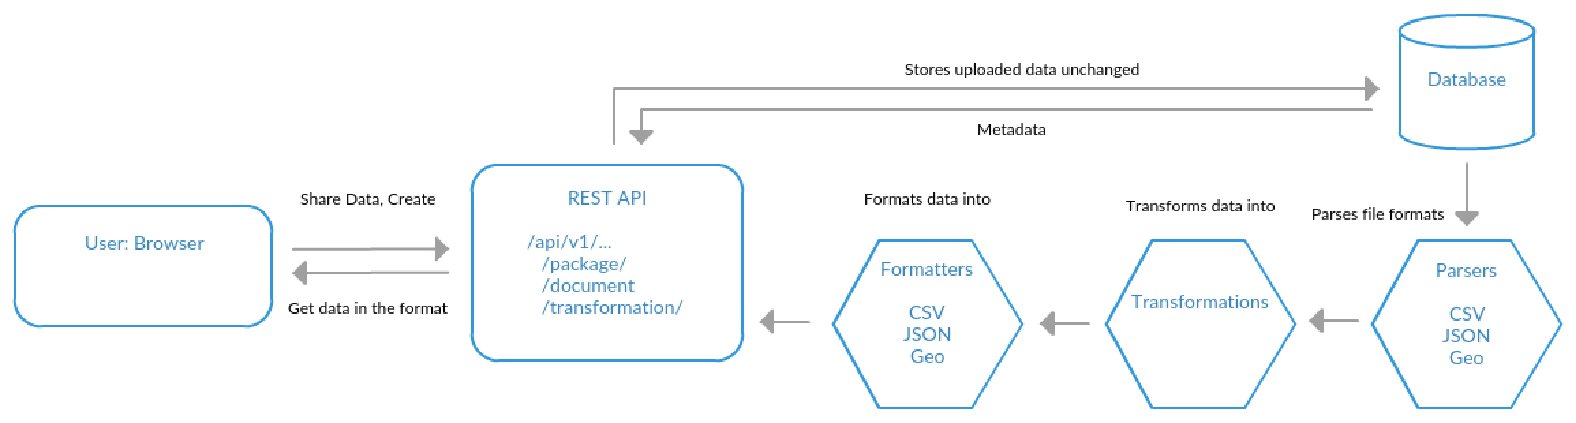
\includegraphics[width=\linewidth]{fig/ODH-Architecture-Overview}
    \caption{Grobe Architektur-Übersicht}
    \label{fig:pd:arch-overview}
\end{figure}

\subsection{Komponenten und Packages}

\begin{figure}[H]
    \centering
    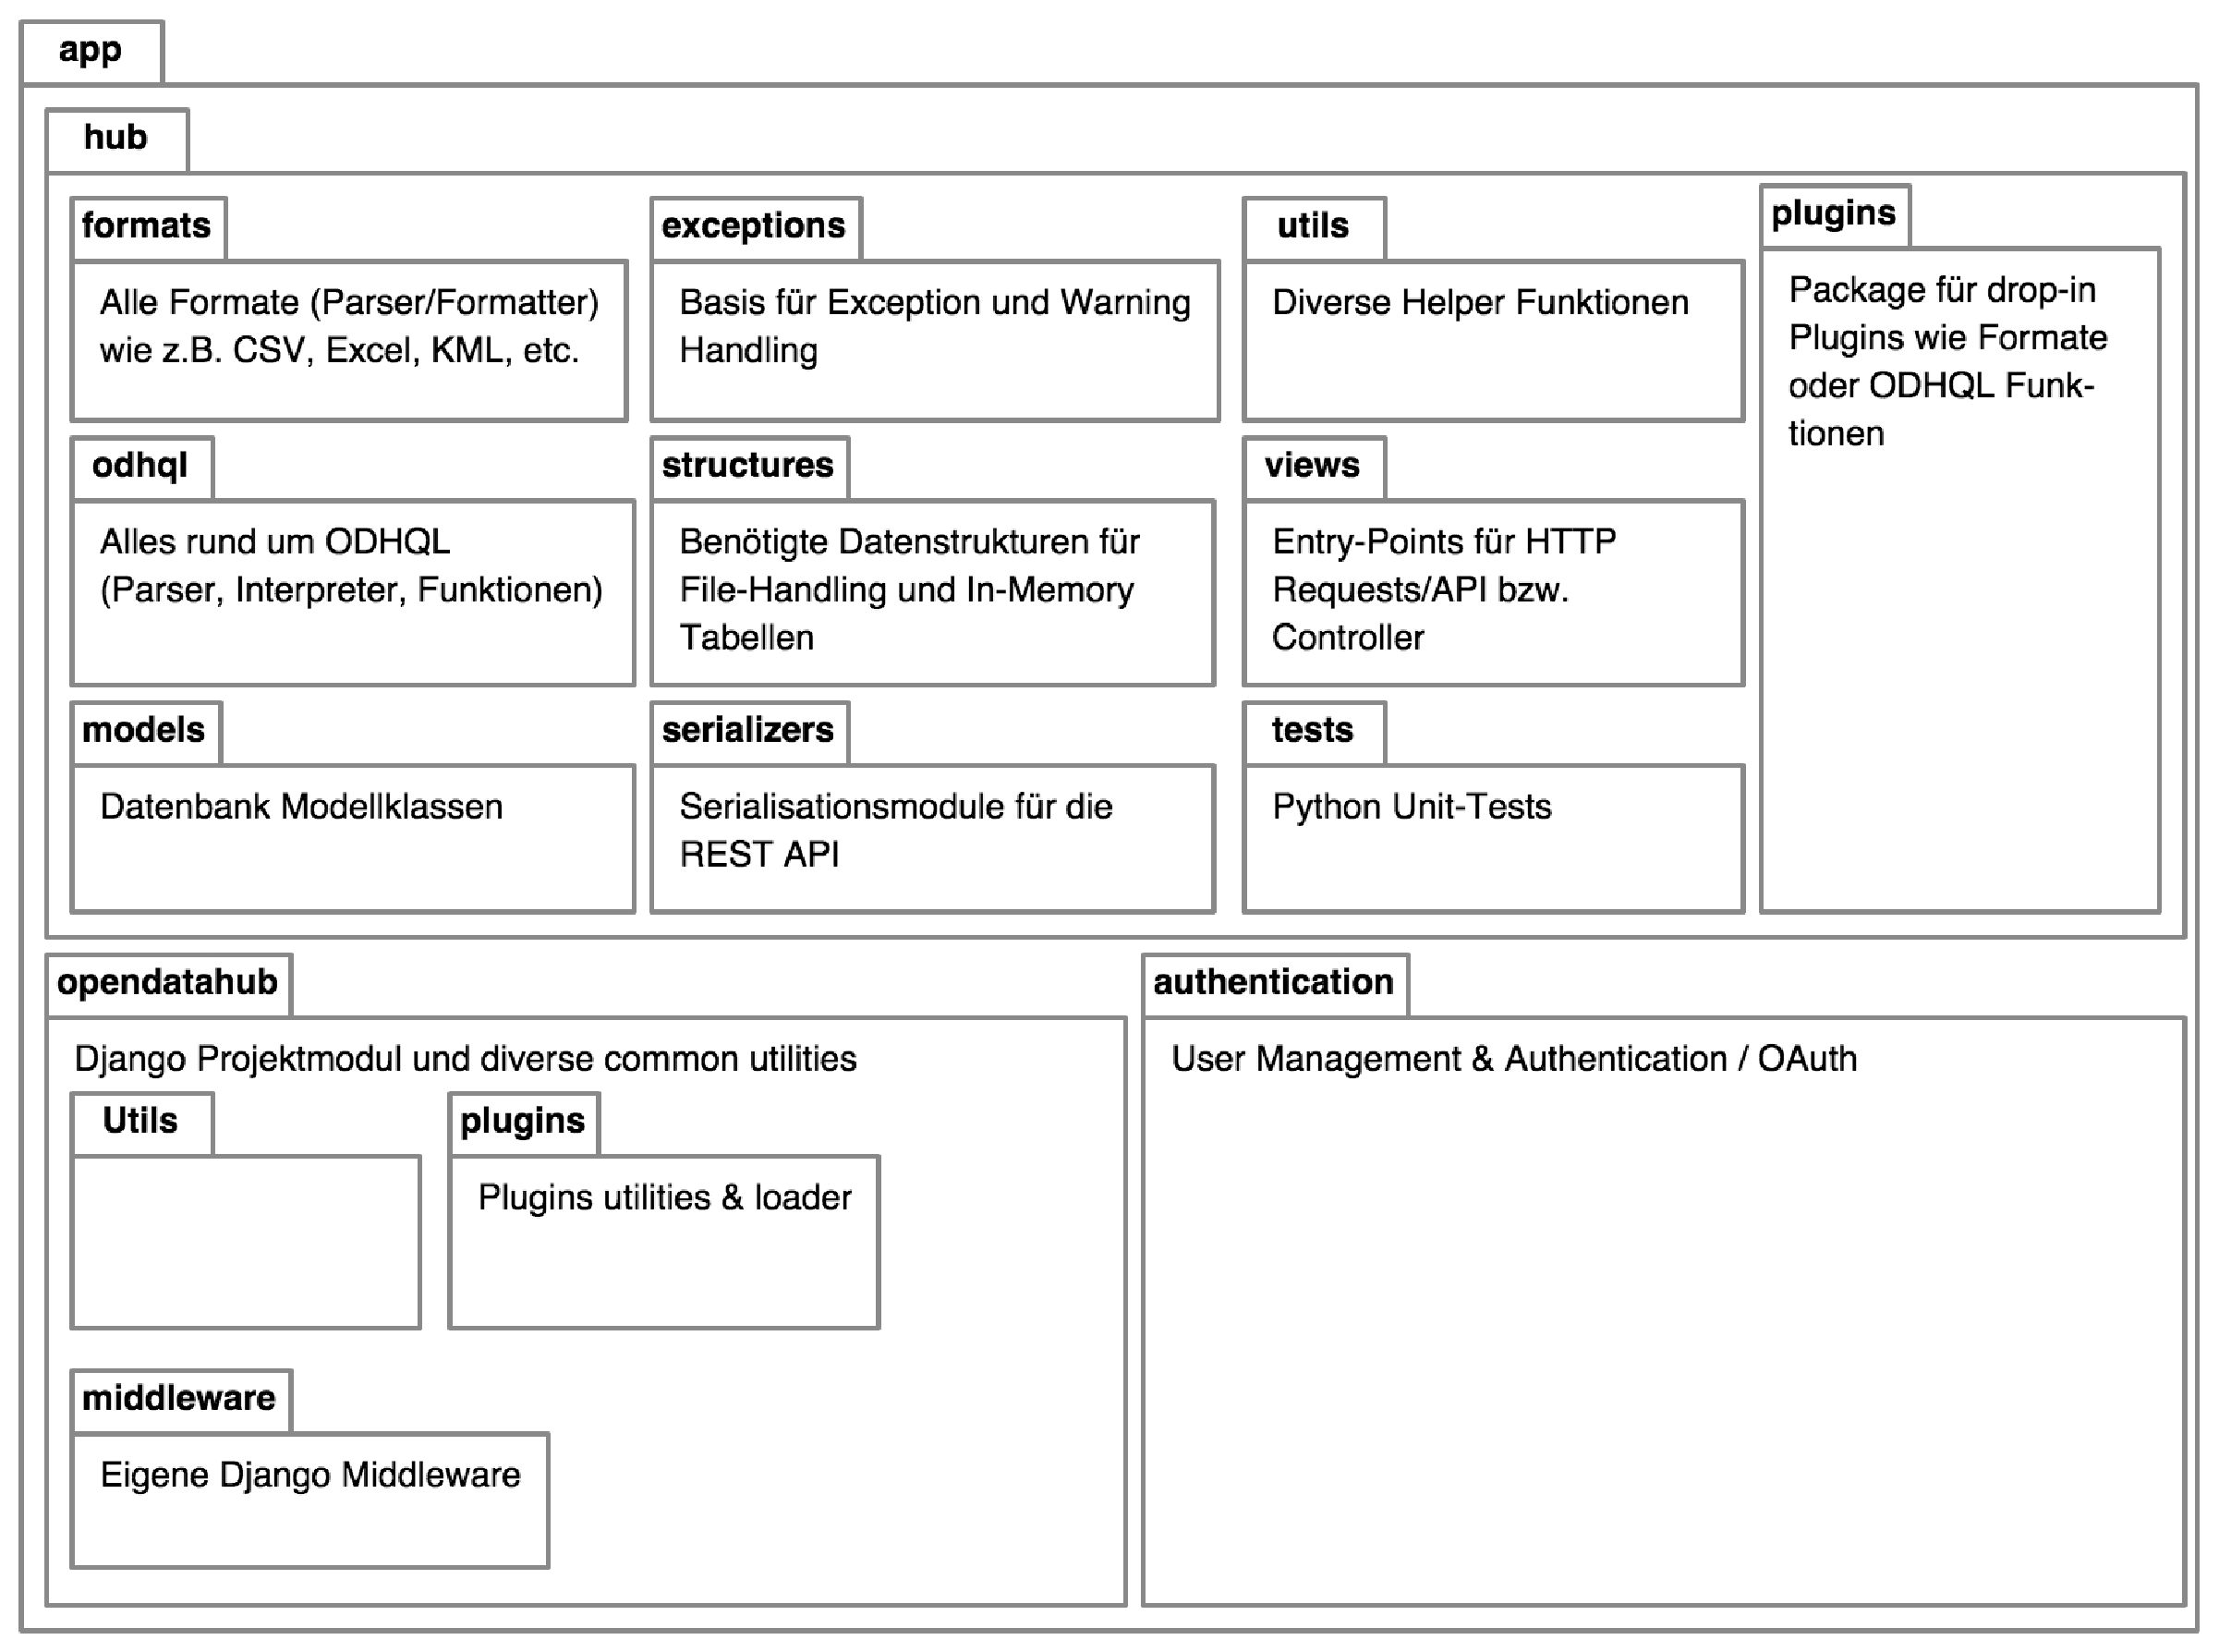
\includegraphics[width=\linewidth]{fig/packages}
    \caption{Python Packages}
    \label{fig:pd:pypackages}
\end{figure}

\subsection{Klassen}


\subsection{Sequenzdiagramm}
